\documentclass[a4paper,11pt]{article}
\usepackage{a4wide,graphicx,amssymb, amstext, amsmath, epstopdf, booktabs, verbatim, geometry, appendix, natbib, lmodern, tabularx, float}

%\geometry{letterpaper}
%\usepackage{garamond}

\newcommand*\Title{Trafic Control System}
\newcommand*\cpiType{Project Plan}
\newcommand*\Author{}
\title{\Title}
\author{}
\date{\today}
%-----------------------------------------------------------

\usepackage{template/template} % This is what makes your document look like a cpi document.


\begin{document}

\begin{titlepage}
\maketitle
\end{titlepage}

  	\linespread{1.15} %Set standard document linespacing
    
  	
  	\tableofcontents
  	\newpage
  	\section{Introduction}
  	The purpose of this document is to describe the overview of the given project. The aim of the Project Plan is to serve as an official contract between the formal client and the team. We, 4Cube, will elaborate the project in details, such as: who the formal client is, their goals, what we will provide to satisfy their requirements and also what we are not obliged to deliver of the client. // In addition we will discus in details the project management such as the cost, time, personnel involved, etc.  
  	
  	\section{Project Statement }
  	\subsection{Formal Client}
  	The formal client of this project is Mr.George. \\ He works in the city of CSharp, in which he is mainly responsible for the traffic situation. \\
  	Our formal client, Mr. George contracted us via his acquittance Mr Peter Massen and Mr. Peter Boots who are both teachers of Fontys. 
  	
    \subsection{Project Leader}
    Agnes Wadee, a Software Engineering student in class Ei7s2, of Fontys University of Applied Sciences will be the project leader. \\ The project leader represents a group of Software Engineering students: 4Cube.
    
    \subsection{Current Situation}  
    In the past few years, the city of CSharp has endured a lot of traffic accidents. The traffic is poorly managed, and therefore, our client, Mr. George aims to place some traffic lights in order to reduce the impact positively in the society by reducing the occurrence  of traffic accidents on the roads.  \\ Based on the overview received from the client about the project, we made a few assumptions. \\ CSharp is a large city with a huge population.\\ There is currently a non-existing application or an existing application which isn't functioning well, in order to assist Mr. George in his tasks.	
    
    \subsection{Project Justification}
    In order to overcome the occurrence of accidents in the city of CSharp, our formal client wants to place traffic lights as a measure. 
    However, idea of just placing traffic lights on the roads without investigating the impact is not optimal.  Therefore, he wants a traffic simulation program with the objective of it being able to simulate the traffic situation. \\
    This traffic simulation software will give information to our formal client about whether it is a good idea to  place the traffic lights and the ideal location to place it.  
    
    \subsection{Project Product}
    The goal of 4Cube Developers is to produce a traffic simulation application for our client. 
    
    \subsection{Project deliverables and non deliverables  }
    In this project we will deliver: 
    \begin{itemize}
    \item A tested and working traffic simulation application.
    \item The source will also be a deliverable
    \item A user manual which outlines the features of the application and guidelines for the user.
    \item A process report.
    \item A Project Plan
    \item User Requirements Specification Document which outlines the technical requirements of the project.
    \item A Design Document which will give an overview of the design of the software.  
    \item Agendas and minutes of every meeting
    \item A Test Plan which elaborates on the tests we have made throughout the application.
    \item A final Presentation about the project.
    \end{itemize}
   
    
    Unfortunately, we will not deliver the following:
    \begin{itemize}
    \item There will be no training organized for the users of the application.
    \item There will be no seminars or talks about the use of the application.
    \item For presentation purposes only, exemplary data will be used, but the client is responsible for the implementation of the actual data. 
    \item Disclaimer: It is not our responsibility to handle the consequential damages as a result of using this application.
    
    \end{itemize}
    
         
       
    \subsection{Project Constraints}
    \textbf{Language}\\The language constraint on this project is \texttt{C\#}.
    \\ The language of the software will be English.
    \\
    \\
     \textbf{Manual}\\The manual will be in PDF.
     \\ The language of the manual will be English.
     \\
     \\
    \textbf{Operating System}\\ The software should run on a computer with Windows running the latest .NET Framework. If the computer runs on Mac OS X, Linux or *BSD, we recommend a Windows virtual machine.
    \\
    \\
    \textbf{Usability}
    \\This application will be a single user application. Multiple users cannot operate with the software at the same time.
    \\ 
    \\
    
    \textbf{Time}
    \\The project has to be completed within 14 weeks.
    
    \subsection{Project Risks}
    \begin{table}[h!]
    \centering
    \caption{Risks Outline.}
    \label{tab:table1}
    \begin{tabularx}{\textwidth}{ |X|X|X|X| }
    \hline
    \textbf{Risk} & \textbf{
   Possibility
	}& \textbf{
Impact
}& \textbf{
Alternative Scenario
}
    \\
    \hline
    Risk of not being able to complete before the deadline	&Low &High&
    Check schedules regularly to ensure we are on schedule.
    \\
    \hline
    Occurrence of application errors & Moderate&High&
    We will test our devices beforehand to avoid any of these occurrences.
    \\
    \hline
    
    Use of legacy software poses a risk since the implementation could be difficult & Low&Low&
    We will write our own code if legacy software is not convenient  
    \\ \hline
    
  
    
    \end{tabularx}
    \end{table}
   \newpage
      \section{Project Phasing}
      Below is an image showing the time phasing of the project, together with the tasks to be performed and the time taken.\\
      The total time taken to complete and deploy the project is 14 weeks, and the breakdown of time is stated below.
      \begin{figure}[h]
      	\centering
      	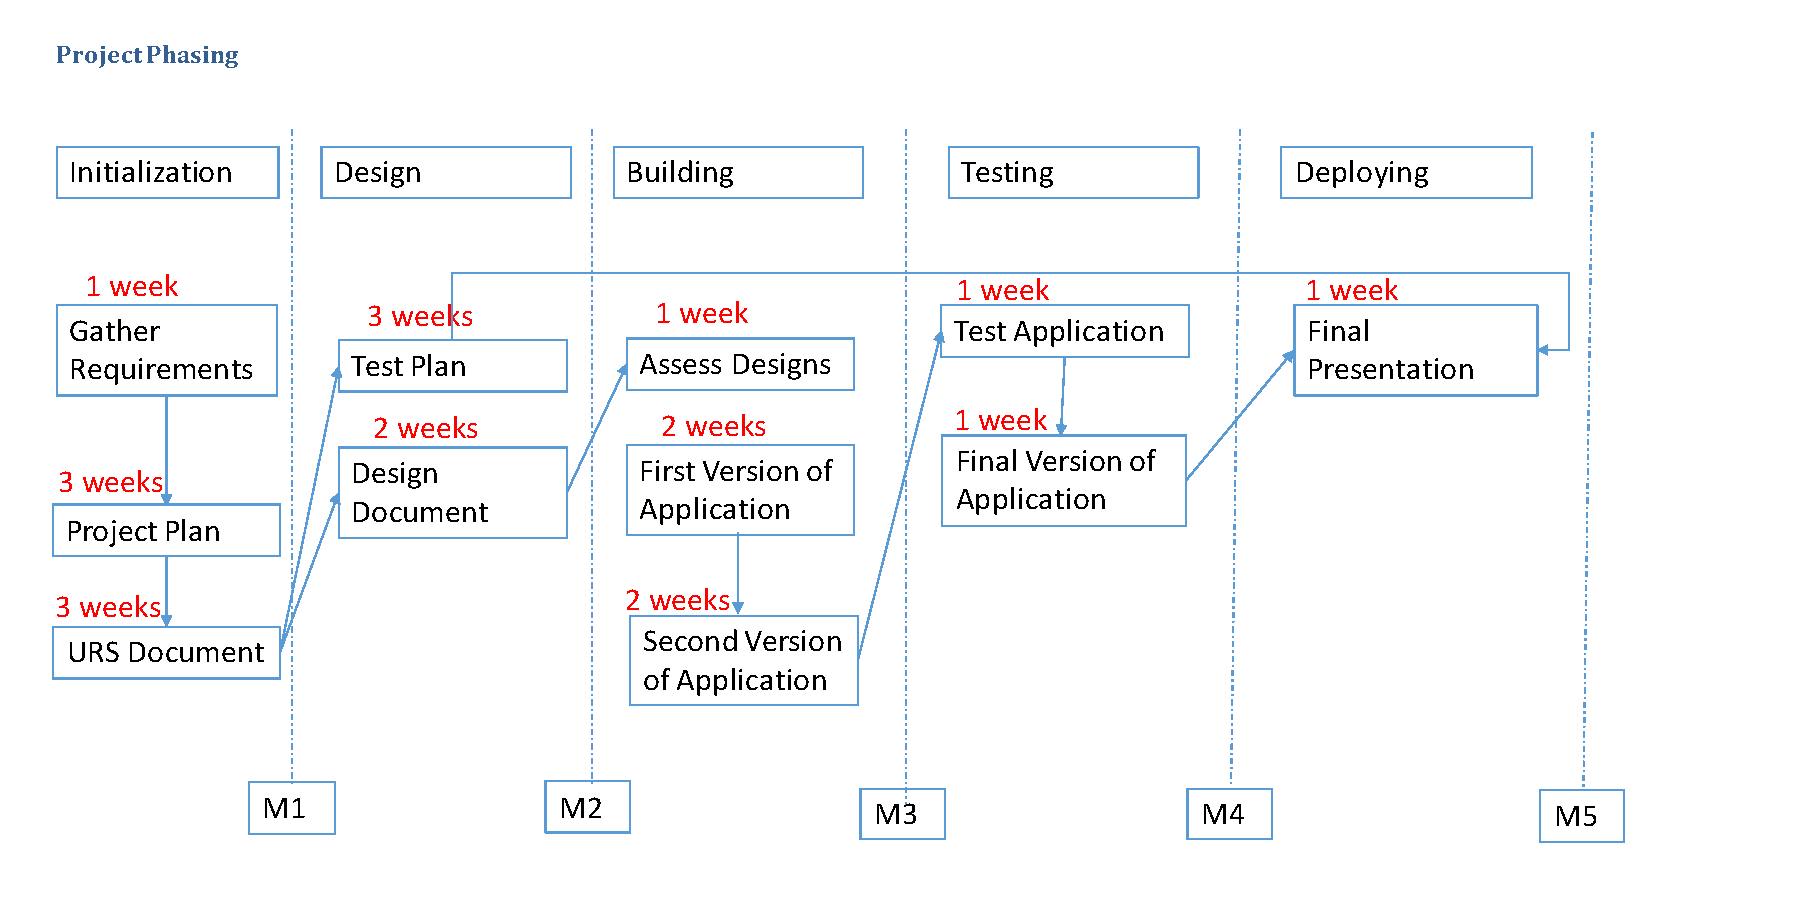
\includegraphics[width=\textwidth]{figures/projectPhasing.pdf}
      	\caption{Project Phasing}
      	\label{fig:pp}
      	\end{figure}
      	
      	\subsection{Deliverables for each milestone}
      	\subsubsection{Milestone M1}
      	  \begin{itemize}
      	  	\item Detailed plan of delegation of tasks for team members.
      	  	\item The Project Plan
      	  	\item Agreement with the formal client concerning the deliverables and non deliverables.
      	  	\item Detailed information outlining the requirements of the application.
      	  	\item URS (User Requirements Specification Document)
      	  	\item Design of Graphic User Interface
      	  	
      	  \end{itemize}
      	  
      		\subsubsection{Milestone M2}
      		\begin{itemize}
      		
      			\item The Test Plan
      			\item The Design Document 
      			\item Final version of Project Plan
      			\item Final version of URS Document 
      		
      	\end{itemize}
      	
      	\subsubsection{Milestone M3}
      	\begin{itemize}
      		\item Working version of the traffic simulation application 
      		
      	\end{itemize}
      		\subsubsection{Milestone M4}
      		\begin{itemize}
      			\item Tested application and a revised version in relation to the tests performed.
      			
      		\end{itemize}
      		
      
      	\subsubsection{Milestone M5}
      	\begin{itemize}
      		\item  Deployment of application and presentation.
      		
      	\end{itemize}
      	
      	\section{Project Management Plan }
      	\subsection{Money}
      	There are no cost involved in making the project, since we are making an application, that does not require, web hosting, neither does it require outsourcing or a special development tool. To build the software, Visual Studio is required, but, we as developers have the educational license.
      	
      	\subsection{Skills}
      	  The project will be performed entirely by the team members of 4Cube consisting of:
      	 \begin{itemize}
      	 	 \item Agnes Wadee
      	 	 \item Coen Stange
      	 	 \item Wen Li
      	 	 \item Yongshi Liang
      	   
      	 \end{itemize}
      	 This team is made up of expertise in the following areas which are beneficial in achieving a successful product.
      	 \begin{itemize}
      	 	\item Project Manager
      	 	\item Software Engineer
      	 	\item Software Architect 
      	 	\item User Interface Designer
      	 	\item Software Tester
      	 	
      	 
      	 \end{itemize} 
      	
      	\subsection{Quality}
      	Being aware of our target audience, we realized that they do not have that much knowledge in ICT. Therefore, we presume a user friendly interface will be ideal to enable them use the application with ease. \\ It is very important to us that our application runs smoothly and efficiently without any bugs. In order to assure this quality, we have a Test Plan made which outlines what we will test for in the software and we will make sure our software runs according to the plan. 
      	
      	\subsection{Information}
      	\begin{table}[h!]
      		\centering
      		\caption{Information Table}
      		\label{tab:table2}
      		\begin{tabularx}{\textwidth}{ |X|X|X|X|X|X|}
      			\hline
      			\textbf{Role} & \textbf{
      			Project Plan
      				}&  \textbf{
      			Minutes
      				}& \textbf{
      				Agenda
      			}& \textbf{
      		Deliverables
      		}& \textbf{
      	Presentation
      	}
      				\\
      				\hline
      			Formal Client&A&R&R&R,A&R,A
      				\\
      				\hline
      				Project Leader& Dr&A&Dr&Dr, A&Dr, A
      				\\
      				\hline
      				
      			Project Team&Di&Dr&Di&Di, Dr & Dr
      				\\ \hline
      				Chairman& Di, A &A&Dr&A,S&-
      				\\ \hline
      				Secretary& S & Dr,S &Di,S&S&-
      				\\ \hline
      				
      				\end{tabularx}
      				\end{table}
      				Legenda:\\ Dr - Draw Up\\
      				Di - Discuss \\
      				A - Approve\\
      				S - Send\\
      				R - Receive
      				
      	\subsection{Time}
      	The duration of the project as stated earlier is 14 weeks. The first 7 weeks will be used to make documentation and the other 7 weeks will be used for the actual implementation. 
      		\begin{table}[h!]
      			\centering
      			\caption{Time Overview}
      			\label{tab:table3}
      			\begin{tabularx}{\textwidth}{ |X|X|X|}
      				\hline
      				\textbf{Activity} & \textbf{
      				Category
      				}&  \textbf{
      			Estimated Time
      			}
      \\
      \hline
      Documenting Project Plan&Documentation& 2 weeks
      \\
      \hline
      Writing URS Document& Documentation& 3 weeks
      \\
      \hline
        Writing Test Plan& Documentation& 3 weeks
        \\
        \hline
    Making Design Document& Documentation& 2 weeks
     \\
     \hline
      Implement first prototype& Application& 2 weeks
       \\
       \hline
         Develop second version& Application & 2 weeks
         \\
         \hline
           Test Application& Application& 1 week
           \\
           \hline
            Final version of Software& Application& 1 week
             \\
             \hline
            
              
              
      
    \end{tabularx}
\end{table}

\subsection{Organization}
There are two types of organizing which will be described in the section. The first type of organization is internally (within the team). It is important to notice that we work in such a way that everyone experiences working in each activity. Figure 2 shows the internal organizational structure\\ 
 \begin{figure}[h]
 	\centering
 	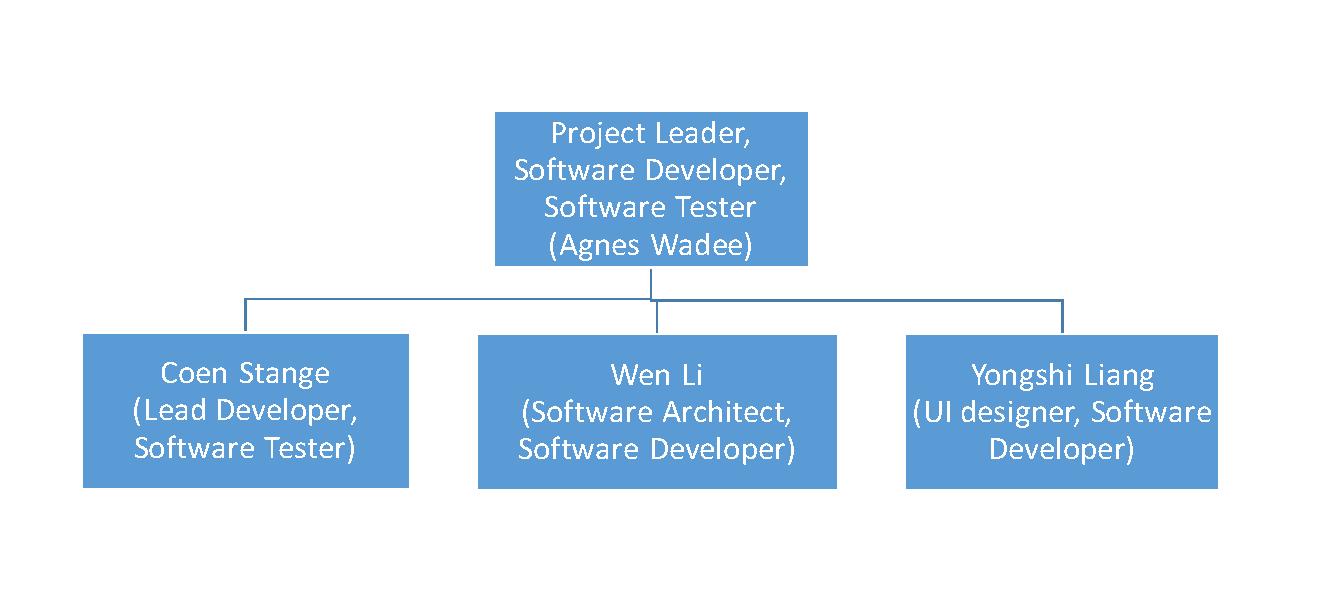
\includegraphics[width=\textwidth]{figures/organization1.pdf}
 	\caption{Internal Organization}
 	\label{fig:Org}
 \end{figure}
 
 
  Whereas, the second type of organization is external.This will outline the communication and relations between the formal client and the team of software developers. Figure 3 shows the hierarchy of each of the parties involved.
 \begin{figure}[h]
 	\centering
 	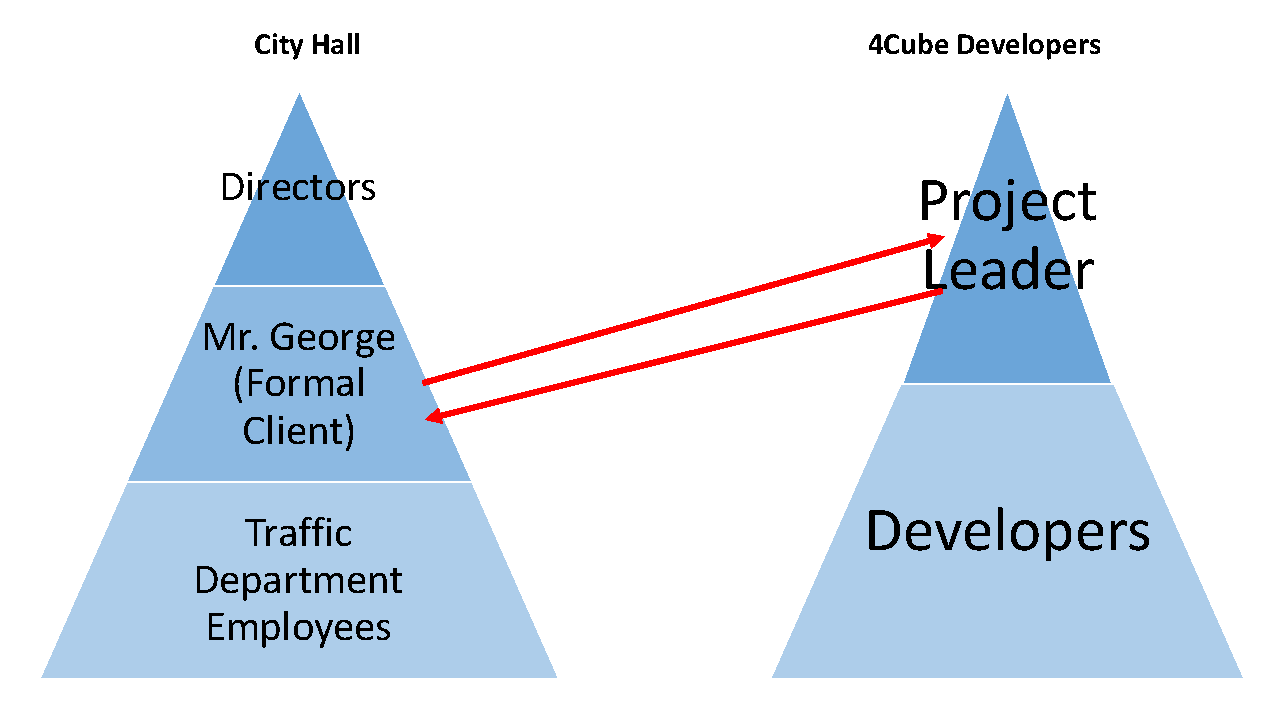
\includegraphics[width=\textwidth]{figures/organization2.pdf}
 	\caption{External Organization}
 	\label{fig:Org2}
 \end{figure}
      	
    \end{document}